\documentclass[12pt,a4paper]{article}
\usepackage[utf8]{inputenc}
\usepackage{graphicx}
\graphicspath{{../Images/}}
\usepackage{amsmath}
\usepackage{amsfonts}
\usepackage{amssymb}
\usepackage{hyperref}
\usepackage[margin=1in]{geometry}
\usepackage{subfig}
\usepackage{float}
\author{Thibaut Marmey}

\title{Titre}
\begin{document}
	\maketitle

\section{Commandes utiles}
\subsection{Listes}
\begin{itemize}
\item
\begin{description}
\item [Changer l'OS par défaut en dual boot :] \hfill \\sudo gedit /etc/default/grub \\GRUB\textunderscore DEFAULT=0 (ubuntu) ou 2 (windows) 
\end{description}
\item Liste des composants de l'ordinateur \textit{lspci}
\newline Pour avoir l'ID des composants : \textit{lspci -nn}
\item Pour régler le problème d'un \textit{sudoers} endommagé : \textit{pkexec visudo}
\item Modifier permission des fichiers : \textit{chmod 754 nomFichier} (owner : RWX, group : R-X, else : R--) 
\begin{center}
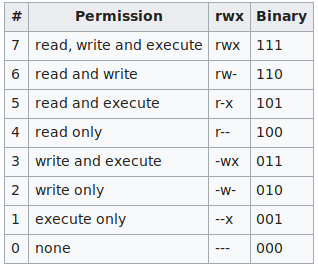
\includegraphics[scale=0.5]{chmod_permission}
\end{center}

\end{itemize}

\end{document}